\documentclass[a4paper,10pt,oneside]{article}
\usepackage{graphicx}
\usepackage{color}
\usepackage{url}
\usepackage{subfigure}
\usepackage[utf8]{inputenc}
\usepackage[T1]{fontenc}
\usepackage{tgpagella}
%\usepackage[scale=0.9]{tgcursor}
%\usepackage[scale=0.9]{tgheros}

\newcommand{\myscale}{0.74}
\newcommand{\vect}[1]{\boldsymbol{#1}}
\newcommand{\code}[1]{\texttt{#1}}
\newcommand{\jmodule}[1]{\emph{#1}}

\setlength{\hoffset}{-1in} %left margin will be 0, as hoffset is by default 1inch
\setlength{\voffset}{-1in} %analogous voffset
\setlength{\oddsidemargin}{1.5cm}
\setlength{\evensidemargin}{1.5cm}
\setlength{\topmargin}{1.5cm}
\setlength{\textheight}{24cm}
\setlength{\textwidth}{18cm}

\def\mftitle{jInfer Architecture}
\def\mfauthor{Michal Klempa, Mário Mikula, Robert Smetana, Michal Švirec, Matej Vitásek}
\def\mfadvisor{RNDr. Irena Mlýnková, Ph.D., Martin Nečaský, Ph.D.}
\def\mfplacedate{Praha, 2011}
\title{\bf\mftitle}
\author{\mfauthor \\ Advisors: \mfadvisor}
\date{\mfplacedate}

\ifx\pdfoutput\undefined\relax\else\pdfinfo{ /Title (\mftitle) /Author (\mfauthor) /Creator (PDFLaTeX) } \fi

\begin{document}
\maketitle
Target audience: developers willing to extend jInfer.\\

\emph{Note: we use the term \textbf{inference} for the act of creation of schema throughout this and other jInfer documents.}\\

The description of jInfer architecture will commence by describing the data
structures, namely representations of regular expressions and XML elements,
attributes and simple data.

Afterwards the interfaces of basic inference modules - \jmodule{Initial Grammar Generator}, \jmodule{Simplifier} and \jmodule{Schema Generator} - will be explained.

Finally, the process of inference will be described.

\section{Package naming conventions}
All packages start with \code{cz.cuni.mff.ksi.jinfer}. Afterwards is the short, normalized name of the module (e.g. \code{base}) and finally the package structure in this module (e.g. \texttt{objects.utils}). All in all, a package in the \jmodule{Base} module could look like \code{cz.cuni.mff.ksi.jinfer.base.objects.utils}.

\section{Data structures}
\subsection{Regular expressions}
For general information on regular expressions, please refer to \cite{wikiregexp}, \cite{automatatheory}.
All classes pertaining to regular expressions can be found in the package \code{cz.cuni.mff.ksi.jinfer.base.regexp}.
In jInfer, we use extended regular expressions as they give us nicer syntax (and easier programming).

Regular expression is implemented as class \code{Regexp<T>} with supplementing classes \code{RegexpInterval} and \code{RegexpType}.
Each \code{Regexp<T>} instance has one of the enum \code{RegexpType} type:
\begin{itemize}
	\item Lambda ($\lambda$) - empty string (also called $\epsilon$ in literature),
	\item Token - a letter of the alphabet,
	\item Concatenation - one or more regular expression in an ordered sequence. Eg. $(a, b, c, d)$,
	\item Alternation - a choice between one or more regular expressions. Eg. $(a | b | c | d)$,
	\item Permutation - shortcut for all possible permutations of regular expressions. Our syntax to write down permutation is $(a\& b\& c\& d)$.
\end{itemize}

Type of regexp is held in \code{type} member in class \code{Regexp<T>} and can be tested by calling methods \code{isLambda()}, \code{isToken()} etc.

Each \code{Regexp<T>} instance has one instance of \code{RegexpInterval} as member.
Class \code{RegexpInterval} represents POSIX-like intervals for expression:
\begin{itemize}
	\item $a\{m,n\}$ means $a$ at least $m$-times, at most $n$-times,
	\item $a\{m,\}$ means at least $m$-times (unbounded).
\end{itemize}
Interval can be either bounded (you have to set both lower and upper bound integers), or unbounded (you have to set only lower bound).
Testing interval value commonly follows routine:
\begin{verbatim}
RegexpInterval i = r.getInterval();
if (i.isUnbounded()) {
  print(i.getMin());
} else {
  print(i.getMin(), i.getMax());
}
\end{verbatim}
That is, first check interval for being unbounded, only if it is bounded, you can ask for maximum.

Class \code{Regexp<T>} can represent regular expression over any alphabet.
This is done by using java generics.
Only token regexps hold instance of type \code{T} in member \code{content}.

Regular expression is in fact $n$-ary tree, for example expression $(a, b, ((c | d), e), f)$ can be viewed as in fig. \ref{reg_tree}.
\begin{figure}
\centering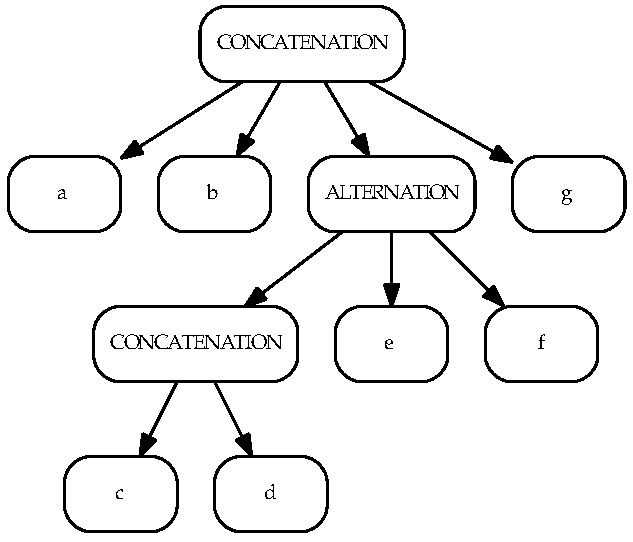
\includegraphics[scale=\myscale]{reg_tree}
\caption{Example tree for regular expression $(a, b, ((c | d), e), f)$} \label{reg_tree}
\end{figure}
We implement this tree by member of \code{Regexp<T>} class called \code{children}, which is of type \code{List<Regexp<T>{}>}.
List contains children of regexp in means of regexp tree.

Regexp has to obey constraits:
\begin{itemize}
	\item type, children and interval have to be non-null references,
	\item when type is lamba, content and interval has to be null,
	\item when type is token, content has to be non-null,
	\item when type concatenation, alternation or permutation, content has to be null.
\end{itemize}
These constraits are checked by constructors, so the best way to construct new regexps is by using 
methods \code{getToken(), getConcatenation()} etc.

Regexp instance is by default created as immutable, that is, once instantiated, you cannot add more children to list of children, cannot change type, content etc. It is to prevent missuse. In special circumstances, one does not know future children of regexp in time of creation. This occurs mainly in input modules, where by parsing XML data sequentially, one does not know contents of element in time of handling start element event.
For these cases, special \code{getMutable()} method is implemented to obtain regexp with none of members set. One has to fill in all properties carefully and call \code{setImmutable()} aftewards. Proper usage should be one of following:
\begin{verbatim}
	Regexp<T> r = Regexp.<T>getMutable();
	r.setInterval(...);
	r.setType(RegexpType.LAMBDA);
	r.setImmutable();cz.cuni.mff.ksi.jinfer.base
\end{verbatim}
\begin{verbatim}
	Regexp<T> r = Regexp.<T>getMutable();
	r.setInterval(...);
	r.setType(RegexpType.TOKEN);
	r.setContent(...)
	r.setImmutable();
\end{verbatim}
\begin{verbatim}
	Regexp<T> r = Regexp.<T>getMutable();
	r.setInterval(...);
	r.setType(RegexpType.CONCATENATION);
	r.addChild(...);
	r.addChild(...);
	r.addChild(...);
	r.setImmutable();
\end{verbatim}
	
Finally, regexp contain one useful method for obtaining all leaves in the regexp tree, it is called \code{getTokens()} and it recursively traverses tree returning list of leaves (token type regexps).

\subsection{XML representation}
XML data basically contains elements, text nodes (characters inside elements) and attributes.
For maximum generality, we decided to break apart theese objects.
We define three basic interfaces: \code{NamedNode}, \code{StructuralNode} and \code{ContentNode} (see package \code{cz.cuni.mff.ksi.jinfer.base.interfaces.nodes}). 

The first stands for bare node in XML document tree, it has its name and context withing the tree (path from root).
The latter two extends \code{NamedNode} interface.
\code{StructuralNode} is for nodes, which form structure of XML document tree: elements and text nodes.
\code{ContentNode} is for nodes, that have content in XML documents: text nodes and attributes.
We have three classes: \code{Element} for elements, \code{SimpleData} for text nodes, \code{Attribute} for attributes (see package \code{cz.cuni.mff.ksi.jinfer.base.objects.nodes}).
In theory, the classes and interfaces would be layed out as on fig. \ref{interfaces_nodes}
\begin{figure}
\centering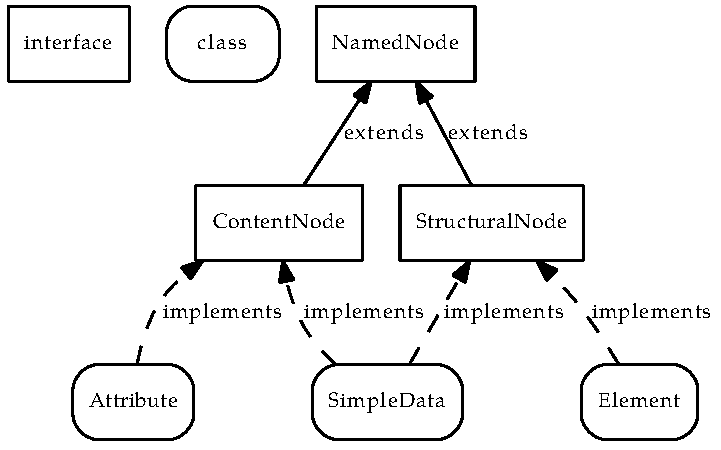
\includegraphics[scale=\myscale]{interfaces_nodes}
\caption{How should interfaces and classes for XML representation look like in theory} \label{interfaces_nodes}
\end{figure}
\begin{figure}
\centering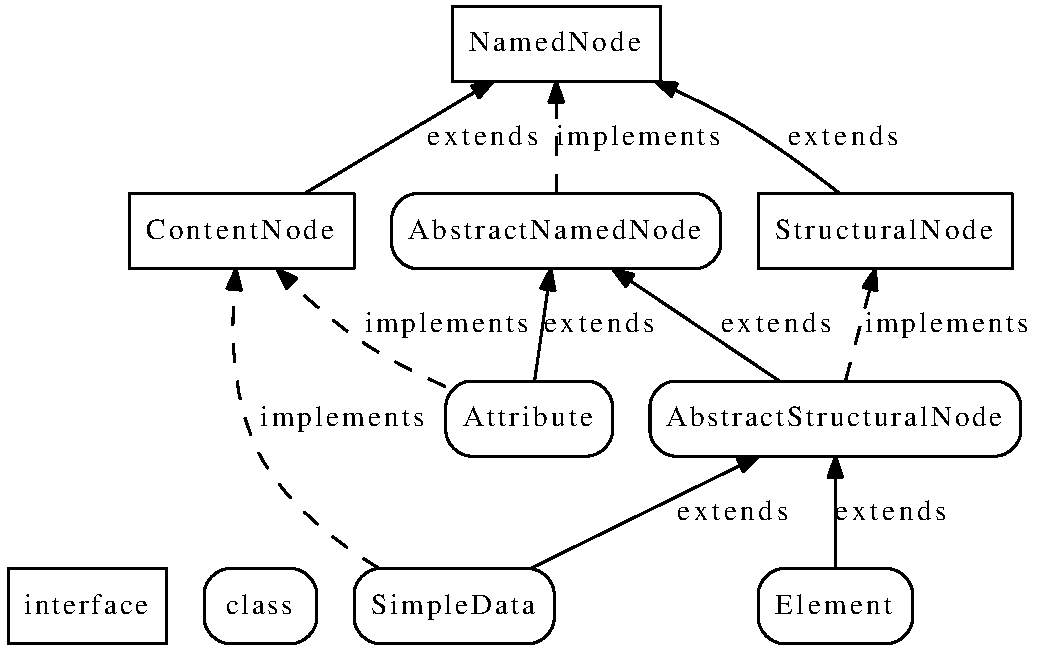
\includegraphics[scale=\myscale]{nodes}
\caption{How are interfaces and classes for XML representation arranged in practice} \label{nodes}
\end{figure}
\begin{figure}
\centering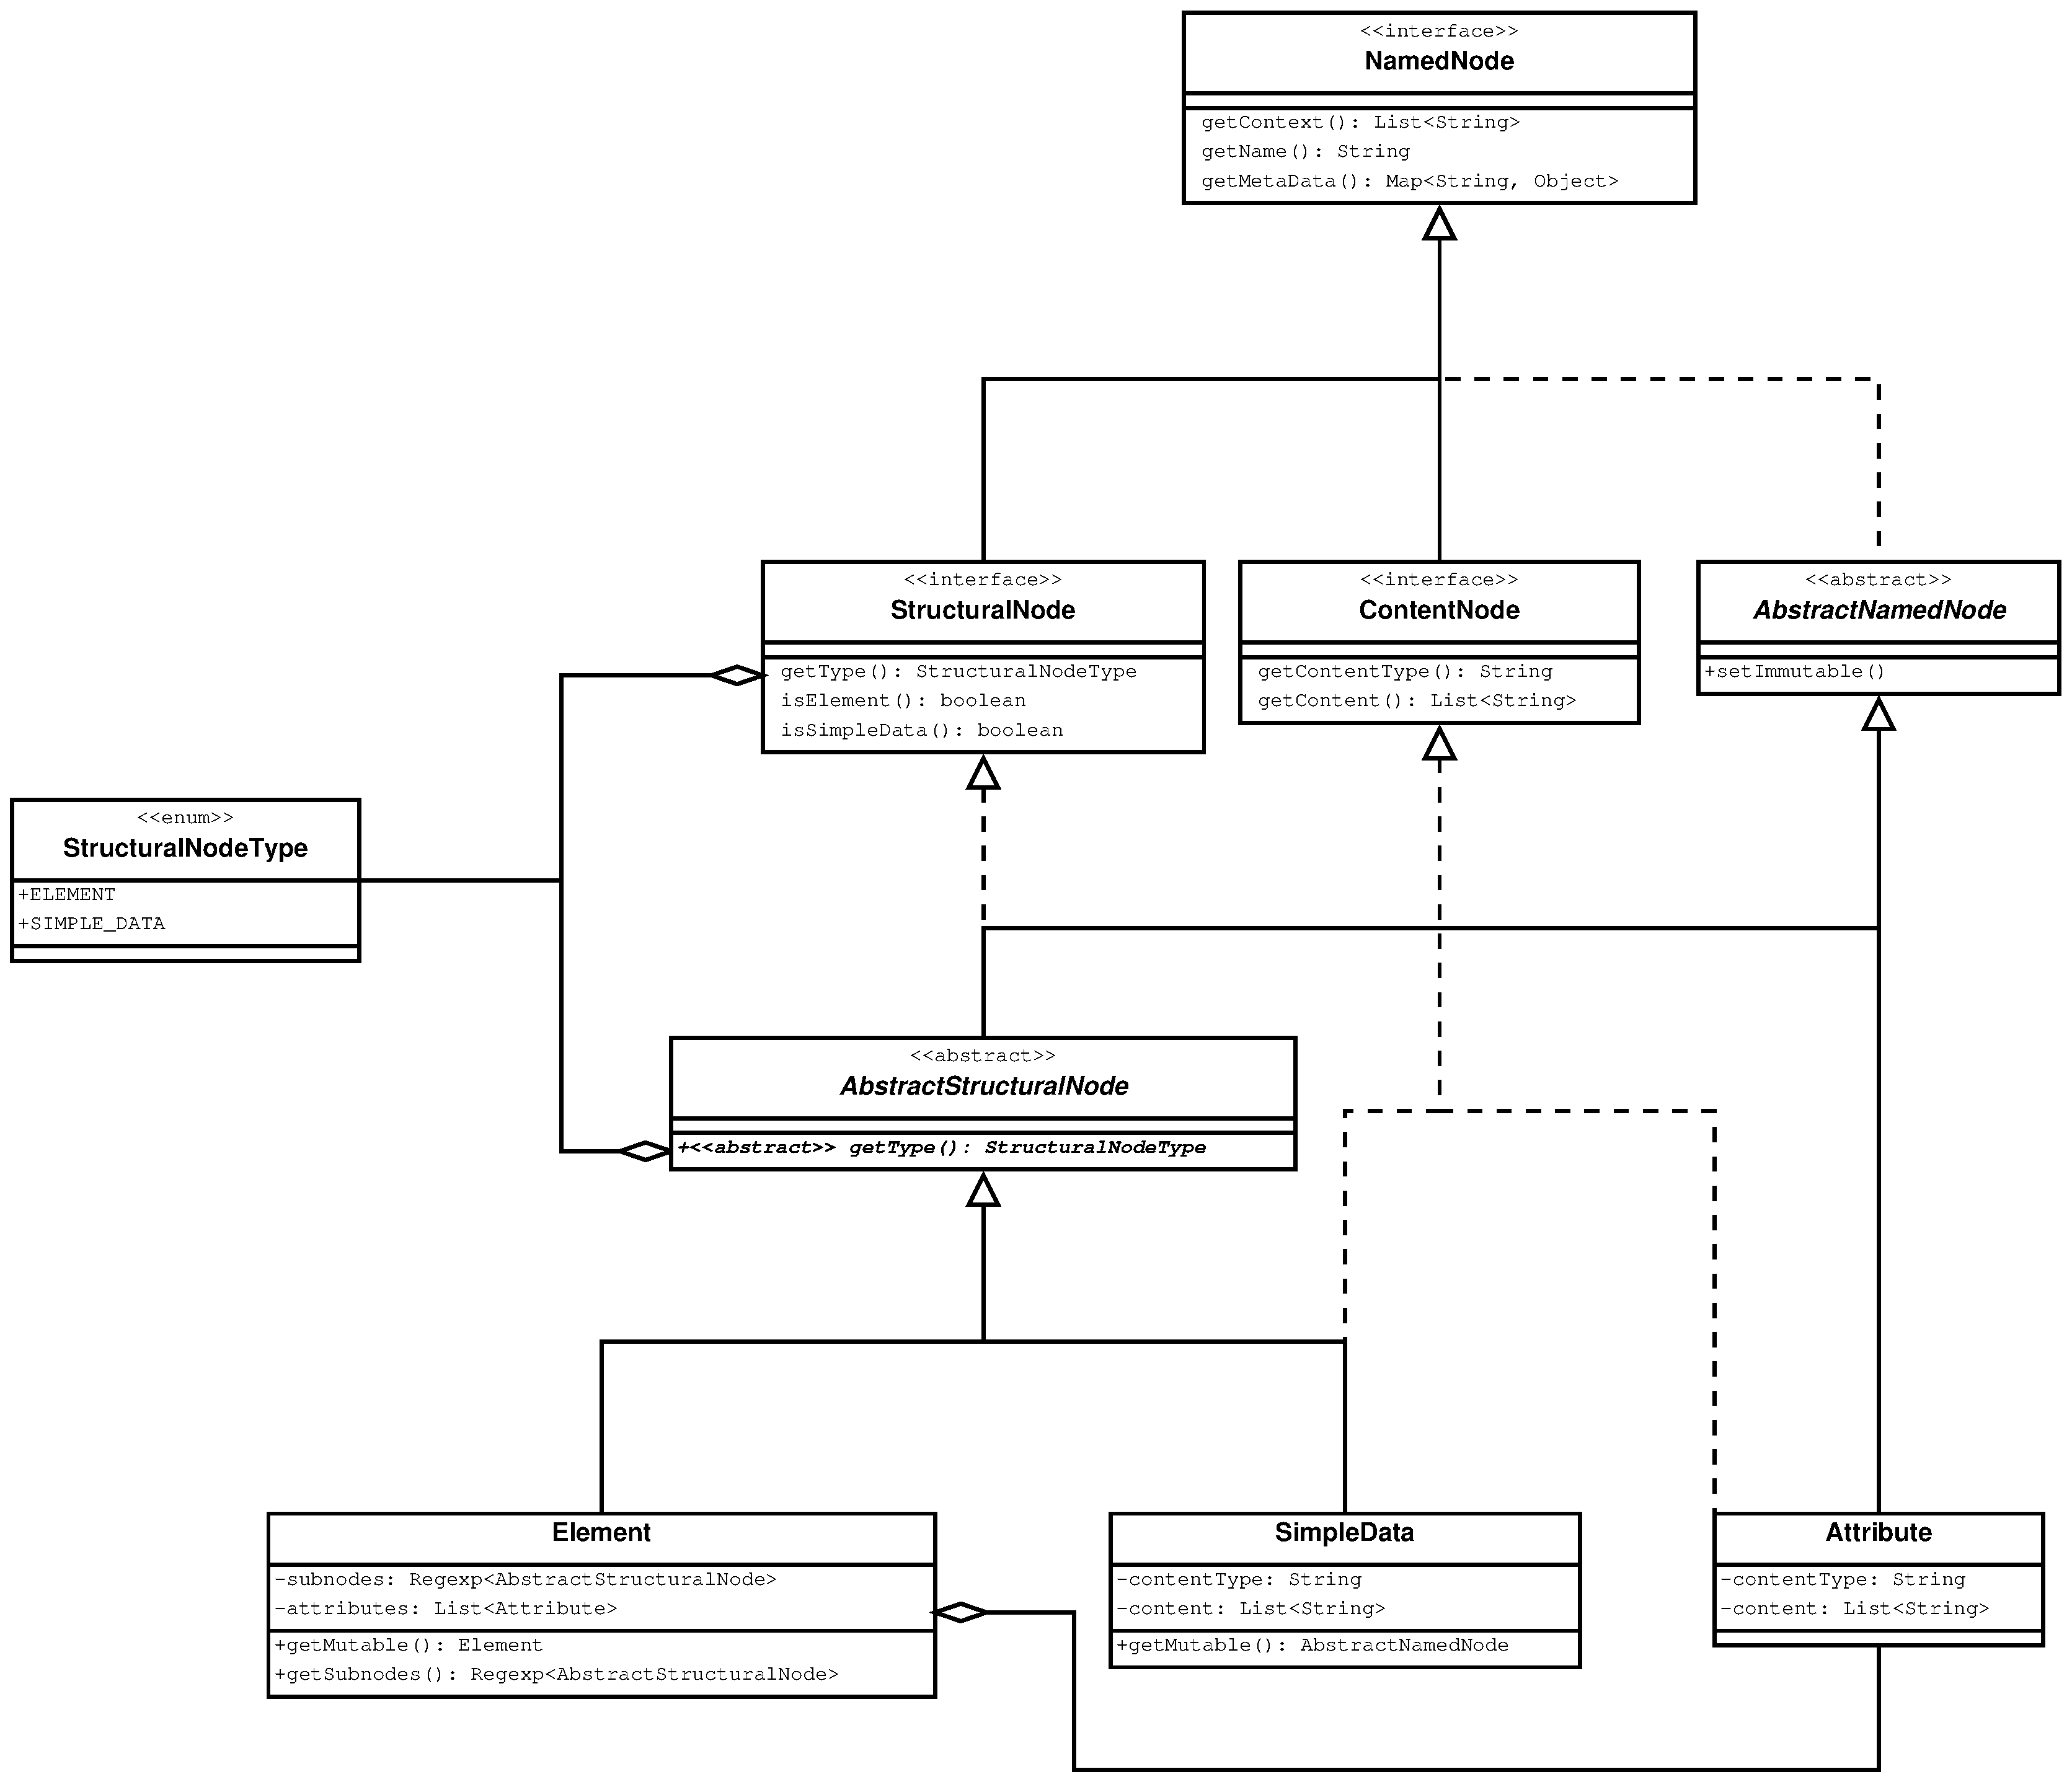
\includegraphics[scale=0.3]{nodes_full}
\caption{XML representing interfaces and classes in detail} \label{nodes_full}
\end{figure}

For even more generality in design, we decided to implement abstract classes in midlevel:
\begin{itemize}
	\item \code{AbstractNamedNode}, which implements methods from \code{NamedNode} interface to handle context, name and metadata (will discuss later in section \ref{section_metada}),
	\item \code{AbstractStructuralNode}, which implements only task of deciding if instance is \code{Element} or \code{SimpleData} actually.
\end{itemize}
As practice showed, for methods handling and infering structural properties, it is important to recognize whether structural node on input is element or text node.
However methods for content devising don't need to know, if they are working on infering model for content of attribute or text node.

Finally, our interface/class model for representing XML nodes is drafted on fig. \ref{nodes}. Those, who are brave enough, can look on fig. \ref{nodes_full}.

In result, \code{Element} and \code{SimpleData} have method \code{getType()} to devise type of \code{AbstractStructuralNode} variables. And \code{SimpleData} and \code{Attribute} have methods \code{getContentType()} and \code{getContent()} to work with content model.

Class \code{Element} has two important members of course:
\begin{itemize}
	\item \code{Regexp<AbstractStructuralNode> subnodes} - for representing right side of grammar rule in resulting infered schema,
	\item \code{List<Attribute> attributes} - for representing all attributes in resulting infered schema.
\end{itemize}
Theese two are filled by import modules, processed further by infering (simplifying) modules and finally exported by exporter modules.

As in regular expressions, classes pertaining XML nodes are by default immutable.
For elements, it means no adding of attributes and changing regexp reference (regexp instance itself is immutable as well).
Same \code{getMutable()} principles and good usage practises as for regexps, hold for theese classes.

\begin{figure}
\centering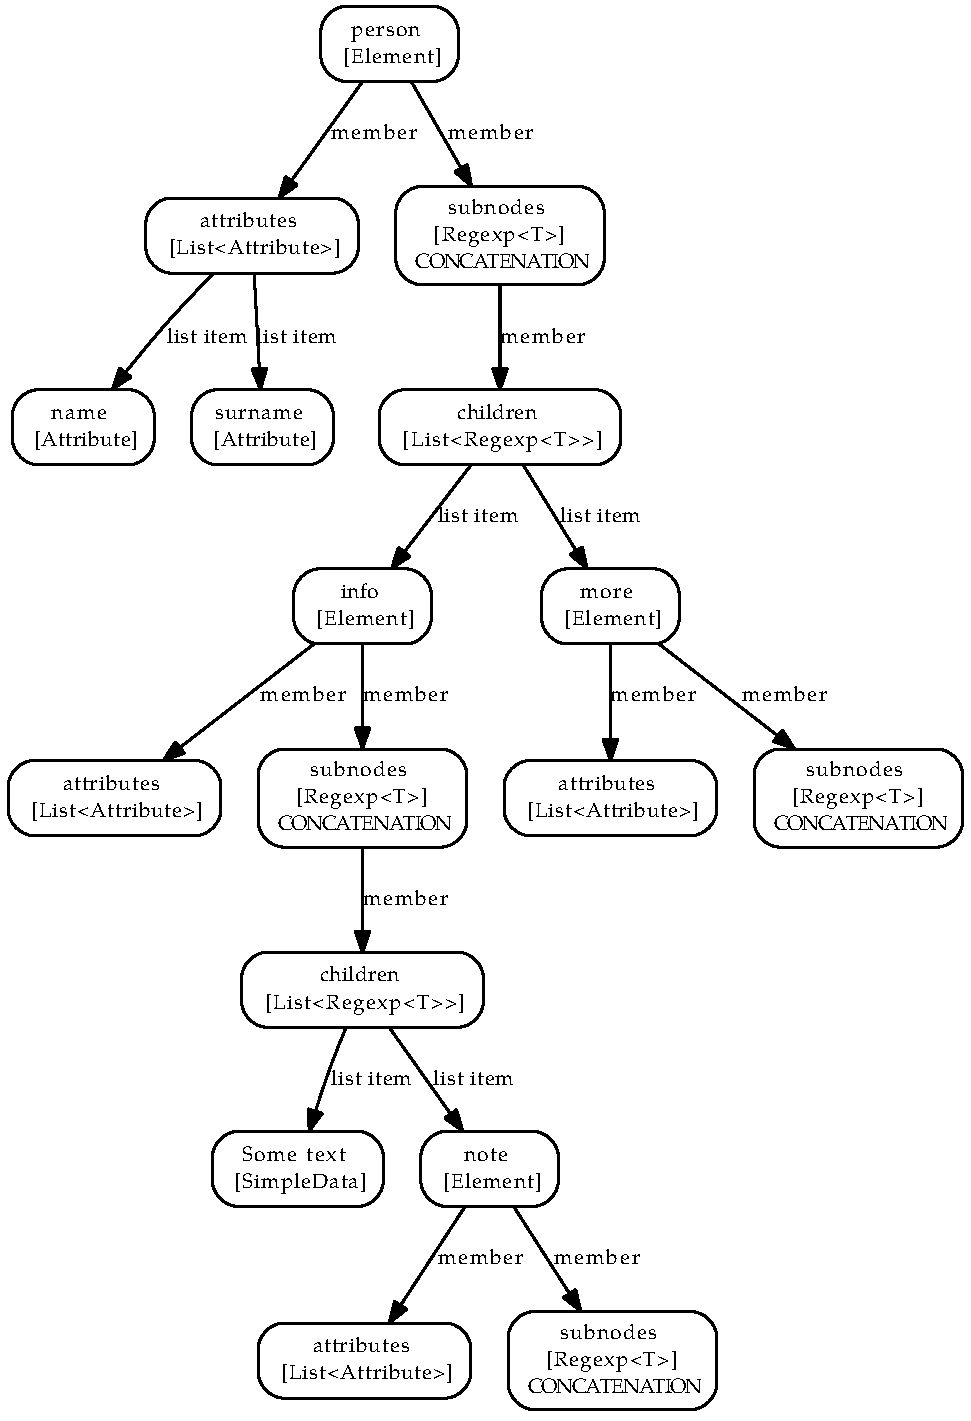
\includegraphics[scale=\myscale]{xml_example}
\caption{XML document representation} \label{xml_example}
\end{figure}
Let's take an example, the following XML document would be represented as tree on fig. \ref{xml_example}.
\begin{verbatim}
  <person name="john" surname="smith">
    <info>
      Some text
      <note/>
    </info>
    <more/>
  </person>
\end{verbatim}
Although in example we present whole document tree, input modules produce slightly different format (consisting of rules).

TODO anti
% hey vektor, what to DO here?

\subsection{Rules, Grammars, etc}

jInfer and its documentation uses extended context-free grammars\cite{extendedcfg}.
% TODO vektor check citation of http://www.engr.mun.ca/~theo/Courses/fm/pub/context-free.pdf in literature.bib
\emph{Rules} in such grammar are in the form
$$
  \textnormal{Left Hand Side (LHS)} \to \textnormal{Right Hand Side (RHS)}
$$
where LHS is a letter of the alphabet (token), RHS is a regular expression over this alphabet. Example would be
$$
  a \to b, (c | d)\ast
$$
In jInfer each such rule is represented with an \code{Element} instance. In this representation, the \code{Element} itself is the LHS, its \code{subnodes} are the RHS.\\

Another important notion is a \emph{grammar}. A grammar consists of its rules, so in jInfer a grammar is just a collection of \code{Element}s. Closely related term is \emph{Initial Grammar}, which for us is a grammar consisting of rules with \emph{simple} right hand sides, i.e. just concatenations of tokens (even with no children, see fig. \ref{xml_example} again). Initial Grammar is produced by \jmodule{Initial Grammar Generator}. % TODO vektor Link

\section{NetBeans Modules}

TODO vektor

\section{Inference process}
\begin{figure}
	\centering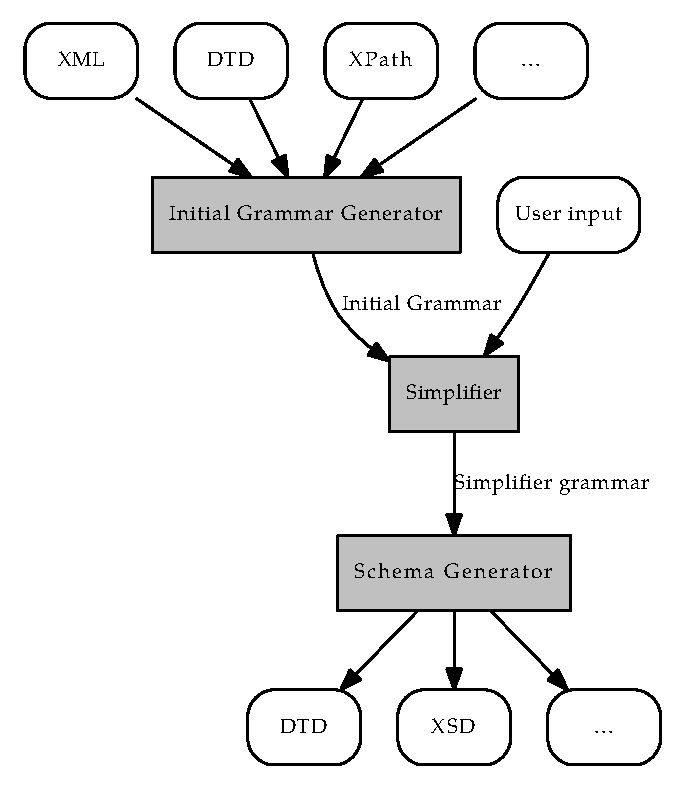
\includegraphics[scale=\myscale]{inference_process}
	\caption{High-level view of the inference process} \label{inference_process}
\end{figure}

The process by which jInfer infers the resulting schema from various inputs (inference process) is summarized by fig. \ref{inference_process}. From the high-level viewpoint, it consists of three consecutive steps carried out by three different modules:
\begin{enumerate}
	\item Initial Grammar (IG) generation: done by the \jmodule{Initial Grammar Generator (IGG)} module, this is the process of converting all of the inputs to IG representation. All documents, schemas and queries selected as input are evaluated, simple rules are extracted and in the end sent to the next step.\\
	For example, a trivial XML document
	\begin{verbatim}
  <a>
    <b>
      <c/>
    </b>
    <d/>
  </a>
	\end{verbatim}
	would translate into the following IG rules
	\begin{eqnarray*}
		a & \to &  b, d \\
		b & \to & c \\
		c & \to & \lambda \\
		d & \to & \lambda 
	\end{eqnarray*}
	\item Simplification: done by the \jmodule{Simplifier} module, this is the process of simplifying, compressing or somehow compactly describing the IG by a smaller number of (more complex) rules (exactly one rule for each element). User interaction might be used in this step to help achieve better simplification. At the end of this step, all rules are sent to the export step.\\
	For example, rules
	\begin{eqnarray*}
		a & \to & b \\
		a & \to & c, d, d, d
	\end{eqnarray*}
	could be simplified to a single rule
	\begin{eqnarray*}
		a & \to & b | (c, d\ast)
	\end{eqnarray*}
	\item Schema export: done by the \jmodule{Schema Generator (SchemaGen)} module, this is the process of actually creating the resulting schema file from the simplified rules. Result of this step is a string representation of the schema, which is sent back to the framework (and later displayed, saved, etc).\\
	% TODO vektor Example
\end{enumerate}
Important thing to note here is that all these steps are executed consecutively. That means, \jmodule{Simplifier} is only started \emph{after} the \jmodule{IGG} completely finished its work and returned IG to be simplified. Similarly, \jmodule{SchemaGen} gets all the rules to export at once, in one list.\\

This modular architecture means that it is possible to replace any and/or all of these modules with \emph{something} else that does similar job. In practice, scientists will probably implement new \jmodule{Simplifier} modules, while using our implementation of BasicIGG and export modules. This modular scheme is used inside our modules to divide them into submodules. It is possible to add new file format processing to import/export. One can extend automaton merging state algorithm of our implementation of \cite{ahonen} in TwoStepSimplifier module by replacing submodules.

% anti : should be after IGG explained, to fulfil is.sentinel explanation i will refer back.
\subsection{Node metadata} \label{section_metadata}
To allow simple extensibility of rules, class \code{AbstractNamedNode} contains a string-addressed map called \code{metadata} that can contain arbitrary object values.\\

At the present, jInfer modules use the following metadata, all defined in \code{IGGUtils} class:
\begin{itemize}
	\item \code{from.schema}, filled in by BasicIGG and XSDImport modules: means that this rule was created (originates from) from a schema.
	\item \code{from.query}, filled in by BasicIGG and XSDImport modules: means that this rule was created from a query.
	\item \code{is.sentinel}, filled in by  BasicIGG and XSDImport module: when importing XML document, one can build whole tree in memory (as in fig. \ref{xml_example}) and then construct list of rules from it (thus saving memory). With schema import however, one not only doesn't know right side of rule in advance (solved by stack in XML import), but right side can be defined anywhere in source file. To save complicated loading of whole schema, searching and pairing elements thorough rules, nodes on right side of rule are created empty - holding only name of node. Fact, that this node has no more information than it's name and position on right side of rule is denominated by labeling the node as sentinel.
	\item \code{schema.data}, filled in by XSDImport module: TODO reseto Explain
	All of these metadata are of set/not set character (using \code{Boolean.TRUE}).
\end{itemize}

% TODO vektor Describe requirements on what gets passed on between modules

\subsection{Nondeterministic Finite Automaton}
For all inference algorithms based on merging states of NFA's, our implementation of nondeterministic finite automaton might be interesting.
Implementation consists of 4 classes: \code{Automaton<T>}, \code{Step<T>}, \code{State<T>} and \code{AutomatonCloner<A, B>} (see package \code{cz.cuni.mff.ksi.jinfer.base.automaton}).
Whole implementation uses java generics for representation of symbol of alphabet, we denote by \code{T} the java type of symbol.

Let's begin by smallest of the classes, the \code{State<T>}.
It represents automaton state, it has two integer members: \code{name} and \code{finalCount}.
Name clearly serves as name of state in visualization and to string conversion.
Final count is for representing whether the state is final in automaton.
The field is not true/false but integral to help algorithms use stastistics over automatons (how many times in XML input is this state final?).

Next we have \code{Step<T>} which stands for automaton transition.
It has its \code{source} and \code{destination} states references.
Symbol accepted by using this transition is store in \code{acceptsSymbol} member of generic type \code{T}.
And finally member \code{useCount}, which is integer stating how many times the transition was used when constructing prefix tree automaton from input data.
Simplifying algorithm can use this number for statistic purposes.

\code{Automaton<T>} class puts theese together into nondeterministic finite automaton.
It has reference to \code{initialState}, it has \code{newStateName} integer value to assure unique state names inside one automaton (incrementing every time new state creates).
We use two maps to implement transition function (delta($\delta$) function  in most literature).
One map of type \code{Map<State<T>, Set<Step<T>>>} called \code{delta} represents mapping from state into set of all outgoing transitions from state.
Second is just reversed map, called \code{reverseDelta}, which holds all incoming transitions into state (for better perfomance).
There exist only one instance of each step from one state to another.
That instance is referenced in delta map (on place of source state), and in reverse delta map (on place of destination state).
Loops are no speciality, just source = destination.

Automaton supports creating automaton as a copy of another one (not reference copy, but true copy), this can be used when searching solution space to create more versions of automaton to edit.
We implemented building of prefix-tree automaton (PTA) in \code{buildPTAOnSymbol()} method.
Create empty automaton and then call this method for every positive example input string of language.
You will get PTA with useCounts and finalCounts set properly on steps/states.

\begin{figure}
	\centering
	\subfigure[Before merge.]
	{
		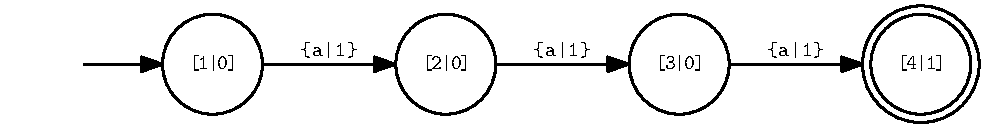
\includegraphics[scale=\myscale]{automaton_merge1}
		\label{automaton_merge1}
	}
	\subfigure[After states 3 and 4 merged.]
	{
		\centering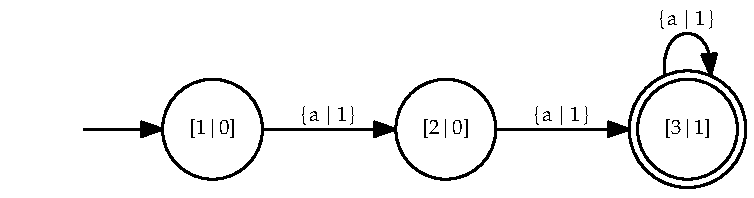
\includegraphics[scale=\myscale]{automaton_merge2}
		\label{automaton_merge2}
	}
	\subfigure[After states 2 and 4 merged.]
	{
		\centering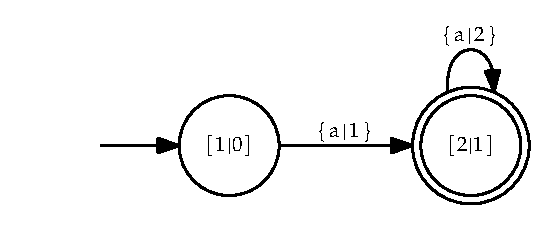
\includegraphics[scale=\myscale]{automaton_merge3}
		\label{automaton_merge3}
	}
	\caption{Sample automaton.} \label{automaton_merge}
\end{figure}

The biggest thing we offer to scientists is state merging by simply calling \code{mergeStates()} method.
Method merges second state given into first one (or all states in list into first one in list).
All \{in | out\}-transitions are redirected properly (or discarted as needed).
Use count and final count are updated as sums of values from merging transitions/states.
One can ask for merging states, that are merged out from automaton already.
Take example automaton of fig. \ref{automaton_merge1} (states are labeled [name|finalCount], steps by \{symbol|useCount\}).
One asks to merge states 3 and 4.
State 3 then becomes final state with loop and state 4 disappears (fig. \ref{automaton_merge2}).
If then one ask to merge states 2 and 4, automaton properly handles situation by knowing, that old state 4, was merged into state 3, and merges states 2 and 3 (see fig. \ref{automaton_merge3}).
This can be useful in $k,h-context$ and $s,k-strings$ implementations (find all context/strings, then supply list of states to merge and don't bother with state names updates).

\subsection{Programmatic view}

From developer's point of view, inference modules are just properly annotated classes implementing one of the following interfaces (all found under \code{cz.cuni.mff.ksi.jinfer.base.interfaces.inference})

\begin{itemize}
	\item \code{IGGenerator}
	\item \code{Simplifier}
	\item \code{SchemaGenerator}
\end{itemize}

A nice way to name such a class is by adding \code{-Impl} to the name of implemented interface, for example \code{SimplifierImpl}.\\

% TODO vektor Connection to NBMs

Annotation required for the framework to recognize such a class as an inference module is the following
\begin{verbatim}
	@ServiceProvider(service = <interface>.class)
\end{verbatim}
for example
\begin{verbatim}
	@ServiceProvider(service = Simplifier.class)
\end{verbatim}

The most important method in each module is \code{start}, defined in each of the interfaces. This method is called by the framework when the respective step of inference is being executed. It has always two parameters: the actual input data for the module, and a callback object to report to when this step is finished. We will look at both parameter now in more detail. 

\subsubsection{Module input}
Each inference module takes the actual input data as the first parameter of its \code{start} method. The type of the argument differs based on the inference module.\\

\emph{Initial Grammar Generator} takes an object of type \emph{Input}. This class encapsulates all the input files in 3 collections of \code{File}: \code{documents}, \code{schemas} and \code{queries}. Enumerating these files provides IGG with access to all data it needs to create Initial Grammar.\\

\emph{Simplifier} and \emph{Schema Generator} take grammar, % TODO vektor Link to grammar definition
in other words a list of rules as input. In the first case, this grammar is the Initial Grammar, in the second case it is the simplified grammar.

\subsubsection{Module output}
Second parameter of each inference module's \code{start} method is a callback object. There are 3 callback interfaces defined in the \code{cz.cuni.mff.ksi.jinfer.base.interfaces.inference} package

\begin{itemize}
	\item \code{IGGeneratorCallback}
	\item \code{SimplifierCallback}
	\item \code{SchemaGeneratorCallback}
\end{itemize}

Each callback interface naturally belongs to the similarly named module interface. As their respective interfaces, also callbacks define one crucial method: \emph{finished}. Each inference module is responsible for invoking this method on the callback it got as a parameter after it has finished its work and has results to be passed on. Again, these 3 finished methods have different arguments based on the inference module.\\

\code{IGGeneratorCallback.finished()} and \code{SimplifierCallback.finished()} have a grammar (Initial Grammar in case of IGG) as their only argument.\\

\code{SchemaGeneratorCallback.finished} has two \code{String}s as arguments: \code{schema} is the actual string representation of the resulting schema, \code{extension} is a file extension of the result (such as "dtd" or "xsd") which the framework will use when saving the result in a file.

\subsubsection{Error handling}

Because the run of each inference module is encapsulated in a \code{try-catch} block by the framework, it is safe to throw any exception out of the \code{start} method: it will get logged, presented to the user and inference will stop. However, if the module uses threads that could throw an exception, it is responsible for catching these exceptions and possibly re-throwing them in the thread where \code{start} runs.

\subsubsection{Interruptions}

User running the inference might change his mind and try to stop this. For this reason, modules have to check for this case in every time-consuming place such as long loops with the following code
\begin{verbatim}
  for (forever) {
    if (Thread.interrupted()) {
      throw new InterruptedException();
    }
    doStuff();
  }
\end{verbatim}

\subsubsection{Runner}

The part of framework responsible for actually gathering user input, running all modules one after another and presenting the results is the \code{Runner} class  in \code{cz.cuni.mff.ksi.jinfer.runner} package.\\

A new instance of \code{Runner} is constructed for each inference run. While being created, \code{Runner}  loads the preferences for current project and looks up user-selected inference modules. Also, callback objects pointing back to methods in \code{Runner} are created. The inference process itself is then as follows

% TODO vektor Picture!!!
\begin{enumerate}
	\item Selected IGG's \code{start} is encapsulated with error/interruption handling and executed, passing \code{Input} and first callback as parameters.
	\item When IGG finishes, it invokes callback's \code{finish} method, passing the IG as parameter.
	\item This in turn causes \code{Runner} to encapsulate and execute Simplifier's \code{start}, passing IG from the first callback and the second callback as parameters.
	\item When Simplifier finishes, it invokes callback's \code{finish} method, passing the simplified grammar as parameter.
	\item This again causes \code{Runner} to encapsulate and execute SchemaGen's \code{start}, passing the simplified grammar from the second callback and the third callback as parameters.
	\item SchemaGen finishes and invokes the last callback's \code{finish}, passing the resulting schema and its extension as parameters.
	\item \code{Runner} receives the resulting schema and based on preferences, saves it to a file, displays it, etc.
\end{enumerate}

% TODO vektor Talk about Capabilities

\nocite{*}
\bibliographystyle{alpha}
\bibliography{literature}

\end{document}
